\chapter{MARCO METODOLÓGICO}
\label{cap:metodo}

\section{Arquitectura del sistema}

La Figura~\ref{fig:diseno} organiza el sistema en dos bloques metodológicos y un
punto de fusión.

\begin{figure}[H]
\centering
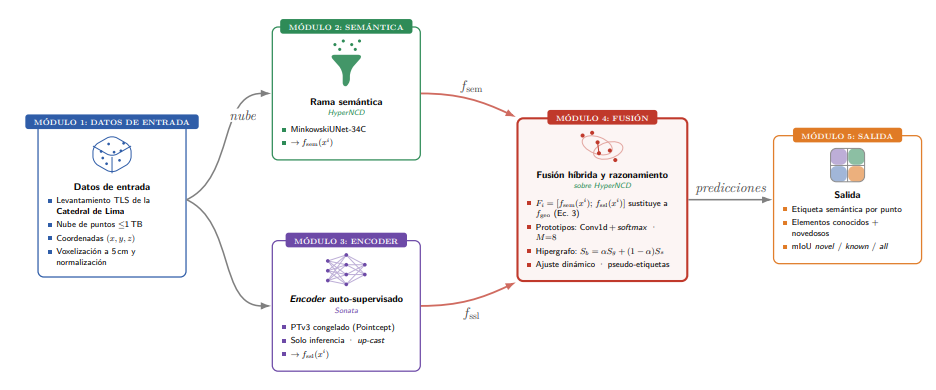
\includegraphics[width=\linewidth]{imagenes/grafico.png}
\caption{Diagrama de diseño del sistema propuesto. La nube TLS de la Catedral de
Lima (Módulo~1) alimenta en paralelo dos ramas de extracción: la rama semántica
MinkowskiUNet-34C de HyperNCD (Módulo~2), que produce $f_{\mathrm{sem}}$, y el
\emph{encoder} PTv3 preentrenado de Sonata (Módulo~3), congelado y usado solo en
inferencia, que produce $f_{\mathrm{ssl}}$. Ambos descriptores entran al
Módulo~4, donde reside el aporte de la tesis: la concatenación
$F_i=[f_{\mathrm{sem}}(x^i);f_{\mathrm{ssl}}(x^i)]$ reemplaza al descriptor
geométrico manual $f_{\mathrm{geo}}$ antes de la formación de prototipos y del
razonamiento por hipergrafo, que permanecen intactos, de modo que la variación de
la métrica sea atribuible al reemplazo.}
\label{fig:diseno}
\end{figure}

El \textbf{Bloque~1} es HyperNCD: aporta la rama semántica (MinkowskiUNet-34C) y
toda la maquinaria de prototipos, hipergrafo dinámico y pseudo-etiquetas que
permite descubrir clases nuevas. El \textbf{Bloque~2} es Sonata: un
\emph{encoder} PTv3 preentrenado de forma auto-supervisada, usado con pesos
congelados y solo en inferencia. El \textbf{nodo de fusión} es el aporte de la
tesis: allí, y solo allí, se sustituye $f_{\mathrm{geo}}$ por $f_{\mathrm{ssl}}$
antes de la formación de prototipos.

\section{Punto de fusión y trazabilidad de la métrica}

Al mover una sola pieza, cualquier variación de la métrica es atribuible al
reemplazo, lo que hace la ablación interpretable sin ambigüedad. Aguas abajo de
la fusión, la afinidad entre prototipos sigue combinando componente geométrica y
semántica según la Ec.~\eqref{eq:afinidad}, y cada prototipo conserva sus $M=8$
vecinos al construir el hipergrafo.

Como el \emph{pipeline} es separable en dos etapas ---inferencia congelada de
Sonata y luego razonamiento de HyperNCD---, la métrica se reporta también en el
punto intermedio y no solo al final: \emph{linear probing} sobre el descriptor
antes de la formación de prototipos (Ec.~\eqref{eq:probe}) y mIoU después
(Ec.~\eqref{eq:miou}). Esa separación es la que permite atribuir una mejora a la
representación o al razonamiento (Sección~\ref{sec:metricas-hibrido}).

\section{Procedimiento experimental}

El procedimiento se ejecuta en cuatro pasos reproducibles. El primero es insumo
de la revisión crítica; los tres restantes corresponden a los objetivos
específicos.

\begin{enumerate}
\item \textbf{Preparación y línea base (Módulo~1).} Teselado de la nube en cinco
secciones disjuntas, voxelización a 5\,cm y normalización; ejecución de HyperNCD
sin modificaciones con tres semillas distintas para fijar el punto de partida de
la Tabla~\ref{tab:base}. El cambio de esquema de normalización fue ensayado y
descartado como resultado negativo (Sección~\ref{sec:linea-base}).
\item \textbf{Fusión (OE1).} Inferencia congelada de Sonata sobre cada sección,
con \emph{cache} de características y \emph{up-cast} para conciliar la resolución
del \emph{encoder} PTv3 con la rejilla de Minkowski; sustitución del descriptor
según la Ec.~\eqref{eq:hibrido} y verificación de funcionamiento de extremo a
extremo sobre una sección de control.
\item \textbf{Calibración (OE2).} Búsqueda por grilla acotada sobre $\alpha$, $M$
y $\epsilon$ en la sección de referencia; la configuración ganadora se congela y
se aplica sin reajuste al resto de secciones.
\item \textbf{Análisis (OE3).} Cómputo de $\Delta$mIoU \emph{novel}
(Ec.~\eqref{eq:delta}), de la brecha cerrada $G$ (Ec.~\eqref{eq:G}) y del
análisis de dominancia (Ec.~\eqref{eq:dominante}), más la ablación de las tres
variantes del descriptor.
\end{enumerate}

\section{Ventaja de dominio del objeto de estudio}

Sonata se preentrenó sobre escenas interiores densas (ScanNet, S3DIS,
Structured3D, HM3D). En LiDAR urbano exterior su \emph{linear probing} queda por
debajo de PTv3 entrenado desde cero (62,0 frente a 69,1 mIoU en SemanticKITTI),
pero en interiores arquitectónicos densos alcanza 72,5 mIoU en ScanNet y 72,3 en
S3DIS Área~5, a la par de modelos supervisados completos. El levantamiento de una
catedral ---estático, denso, de geometría arquitectónica--- cae del lado
favorable de esa frontera, lo que reduce sustancialmente el principal riesgo de
transferencia de dominio.

\section{Riesgos y mitigación}
\label{sec:riesgos}

\paragraph*{(i) Disponibilidad de la nube anotada.} NCD exige al menos las clases
conocidas etiquetadas. Se asume la anotación manual de una sección de referencia
con $\geq$4 clases base; si el levantamiento llega sin etiquetas, esa anotación
se vuelve tarea previa del cronograma y condiciona el inicio de OE1.

\paragraph*{(ii) Acceso y configuración del clúster.} La configuración de GPU de
Khipu ha cambiado respecto de la documentada previamente. Por ello el proyecto no
estima tiempos de calendario: verifica empíricamente el hardware asignado
(Tabla~\ref{tab:hardware}) y fija a partir de esa verificación el tamaño de
ventana y el esquema de \emph{cache}. El seccionamiento de la catedral es el
mecanismo que sostiene el respaldo: ninguna etapa requiere la nube completa en
memoria.

\paragraph*{(iii) Sustitución frente a concatenación (Plan~B).} Si el reemplazo
directo degrada el rendimiento, la variante es concatenar
$F_i=[f_{\mathrm{sem}};f_{\mathrm{geo}};f_{\mathrm{ssl}}]$, dejando que el módulo
de prototipos pondere las tres fuentes. Cualquier resultado ---mejora, paridad o
degradación--- documentado con ablación es reportable.
